\chapter{Présentation de l'organisme d'acceuil et cadrage du projet}
\label{sec:pré}
\section{Introduction}



\medskip

Ce chapitre présente Capgemini Engineering, une société de conseil spécialisée dans les solutions d'ingénierie, ainsi que l'équipe que j'ai intégrée et mon rôle dans le développement d'un système avancé d'aide à la conduite (ADAS) qui fonctionne efficacement dans des conditions météorologiques extrêmes.

Ce projet pose des défis uniques à cause de l'exclusivité de la technique et du nombre limité de publications disponibles sur le sujet. Cependant, il offre également des opportunités significatives de se plonger dans des domaines de pointe tels que la théorie du contrôle, l'apprentissage automatique et l'apprentissage profond. 

Ce chapitre encadre le projet et fournit un contexte permettant au lecteur de comprendre ses objectifs, sa portée et ses résultats attendus, ainsi que le rôle de Capgemini Engineering dans son développement.
\medskip
\section{Présentation de l'organisme d'accueil}
\subsection{Capgemini Engineering}
Capgemini Engineering est une filiale du groupe Capgemini qui rassemble les services
d'ingénierie et de R\&D de Capgemini Engineering, avec un chiffre d'affaires de 16 milliards
d’euros. L'expertise de Capgemini dans le domaine de production numérique ainsi que sa
connaissance sectorielle approfondie lui permettent d'accompagner les entreprises dans leur
transformation vers la 4.0 en conjuguant les mondes physique et numérique. Avec plus de 52
000 ingénieurs et scientifiques dans plus de 30 pays , Capgemini Engineering intervient dans
des secteurs variés tels que l'aéronautique, l'automobile, les sciences de la vie ou encore
l'énergie. Le groupe Capgemini, quant à lui, est un leader mondial responsable et multiculturel
comptant près de 270 000 collaborateurs dans une cinquantaine de pays. Grâce à son expertise
et son expérience, il répond à l'ensemble des besoins de ses clients, de la stratégie à la gestion
des opérations, en utilisant les dernières innovations technologiques. 
\begin{figure}[hbt!]
  \centering
  
\includegraphics[width=0.4\textwidth]{logo.png}
  \caption{Logo de la société Capgemini Engineering}
\end{figure}

En tant que partenaire stratégique, Capgemini Engineering joue un rôle essentiel dans l'accompagnement complet des projets de ses clients à travers divers secteurs industriels.
L'entreprise s'engage à fournir un niveau de service constant et de qualité, en offrant une
expertise approfondie dans chaque domaine.
Afin de répondre aux besoins spécifiques de ses clients, Capgemini Engineering adopte une
approche à la fois mondiale et locale. En tant que groupe d'envergure mondiale, il est en mesure
de proposer des solutions globales et innovantes qui répondent aux défis de l'industrie à grande
échelle. Cependant, il ne perd pas de vue l'importance d'une présence locale et d'une
compréhension approfondie des marchés spécifiques. Cela permet à Capgemini Engineering
d'offrir un accompagnement personnalisé et adapté aux exigences particulières de chaque
marché. Les clients et partenaires stratégiques de Capgemini Engineering jouent un rôle clé
dans la réussite de l'entreprise. En collaborant étroitement avec ces acteurs majeurs de
l'industrie, elle favorise l'innovation, la co-création et la recherche de solutions technologiques
avancées. Grâce à ces partenariats solides, l'entreprise est en mesure d'anticiper les tendances
du marché et de proposer des solutions différenciées qui répondent aux besoins changeants de
ses clients.
\section{Le projet RT-SIM}
L’équipe RT-SIM est composé de cinq docteurs et quatre stagiaires
(moi y compris). Le projet de recherche interne, RT-SIM, a pour but de développer
une plateforme de simulation générique, distribué et temps réel.
\subsection{Contexte}
De nos jours, le développement d’un nouveau produit dans le secteur des transports,
de l’industrie, de l’énergie et bien d’autres est devenu complexe. On souhaite
améliorer la qualité d’un produit en y intégrant de nouvelles technologies, tout en
diminuant le coût et le temps de développement.
C’est ainsi que ces dernières années, il y eut un intérêt croissant pour la simulation.
En effet, les simulateurs permettent d’intervenir sur tout le cycle en V d’un produit
et permettent ainsi d’intégrer de nouvelles technologies tout en diminuant les
coûts et le temps de développement. Les simulateurs devenant de plus en plus
réalistes, il devient de moins en moins nécessaire de développer des prototypes.
C’est ainsi qu’est né le projet RT-SIM qui souhaitait prendre en compte les nouvelles
technologies dans le développement de sa plateforme de simulation, les contraintes
imposés dans les secteurs simulés et la capacité d’être compatible dans tous les
domaines afin de pouvoir rendre un simulateur le plus réaliste possible.
\subsection{objectif}
L’objectif du projet RT-SIM est d’être :
\begin{enumerate}
  \item Générique afin de faire coexister plusieurs secteurs d’activité.
  \item Interopérable avec différents standards (ED-247 et FMI pour l’aéronautique,
  SMP2 pour le spatial, etc.), protocoles de bus de communication (CAN, ED-247,
  AFDX, etc.) et techniques de modélisation (discret et continu).
  \item Distribué avec diverses ressources informatiques connectées par Ethernet.
  \begin{figure}[hbt!]
    \centering
    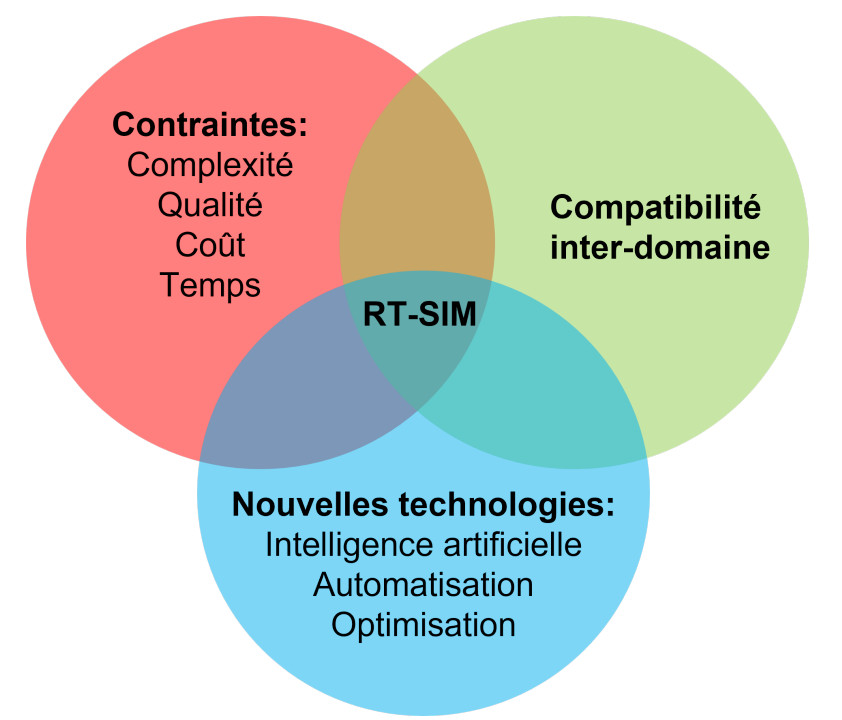
\includegraphics[width=0.5\textwidth]{2.png}
    \caption{Les motivations du projet RT-SIM}
  \end{figure}
  \item Hybride pour faire coexister ”hardware” et ”software”.
  \item Temps réel afin qu'on fassent des simulations HIL (Hardware in the loop).
\end{enumerate}
\begin{figure}[hbt!]
  \centering
  \includegraphics[width=0.5\textwidth]{3.png}
  \caption{Concept du projet RT-SIM}
\end{figure}
\section{Conclusion}

Pour conclure, dans ce chapitre nous avons présenté l’organisme d’accueil \textbf{ Capgemini Engineering} où ce projet a été réalisé, son historique, son organigramme et l’équipe de
travail. En utilisant des différents outils, nous avons mis en évidence le cadre du projet, les
objectifs visés, la démarche de travail et la planification de ce présent projet.
\\
Après, on a montré les limitations causant la problématique traitée dans ce projet, et en comparant les solutions physiques nous avons abouti à la solution physique adoptée dans ce projet.

\medskip
Dans le chapitre suivant, nous allons traiter la partie théorique de RADAR, comprendre le fonctionnement, le traitement de signal nécessaire, et la nature des données récupérées à la fin.\\
Ainsi que la motivation autour l'utilisation de l'apprentissage profond, et une définition de l'architecture des réseaux de neurones (NN).


%%% Local Variables: 
%%% m. Nous avons aussi ode: latex
%%% TeX-master: "isae-report-template"
%%% End: 